\documentclass{amsart}
\usepackage{graphicx}
\usepackage{caption}
\usepackage{subcaption}
\graphicspath{ {./img/} }

\usepackage{pgfplots}
\pgfplotsset{compat=1.18}
\usepackage{wrapfig}

\title{CSE305 - Assignment 1}
\author{Doan Dai Nguyen}

\begin{document}

\maketitle

In this first assignment, I have implemented a raytracer with the following features:
\begin{enumerate}
    \item Surfaces with diffusion, reflection, refraction, and Schlick's approximation of Fresnel's law for better refraction;
    \item Direct lighting, point light source and shadowing;
    \item Indirect lighting, spherical light source, and soft shadowing;
    \item Antialiasing;
    \item Focus of camera and depth of field;
    \item Ray-mesh intersection with BVH;
    \item Phong interpolation.
\end{enumerate}

The assignment was done in 816 lines of code, including 79 lines of code in \texttt{main.cpp} and 737 lines of code from 7 files in \texttt{./classes}. The project was compiled with C++20, and the following compiler flags

\texttt{-fopenmp -O3 -fcf-protection=none -march=native -mtune=native \\-fno-math-errno}

The rendering was done one a laptop with Intel Core i7-10710 CPU, 12 cores with 1.6 GHz. No GPU was used for the rendering in this report.

All pictures below were rendered with 64 rays per pixels.

\begin{figure}
     \centering
     \begin{subfigure}[b]{0.49\textwidth}
         \centering
         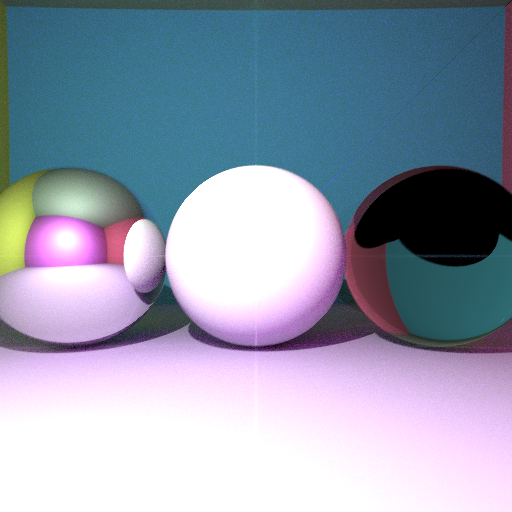
\includegraphics[width=\textwidth]{img/fig1_1.png}
         \caption{Snell's law (9.01 seconds)}
     \end{subfigure}
     \hfill
     \begin{subfigure}[b]{0.49\textwidth}
         \centering
         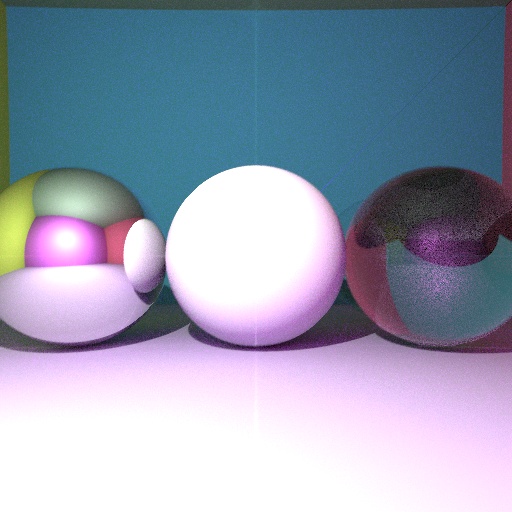
\includegraphics[width=\textwidth]{img/fig1_2.png}
         \caption{Fresnel's law (11.547 seconds)}
     \end{subfigure}
     \caption{Three balls with reflection, diffusion, and refraction. In this picture, the light source was a point.}
\end{figure}

\begin{figure}
     \centering
     \begin{subfigure}[b]{0.49\textwidth}
         \centering
         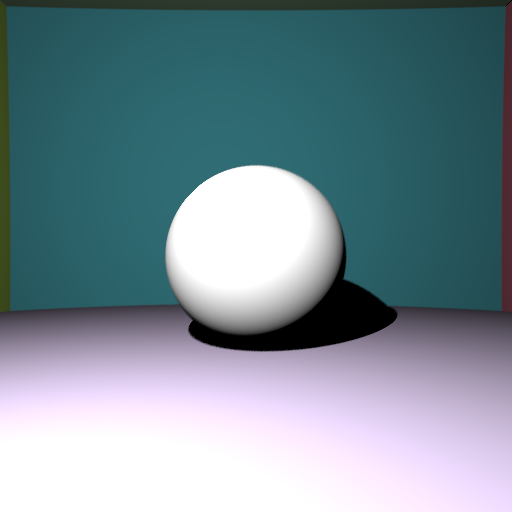
\includegraphics[width=\textwidth]{img/fig2_1.png}
         \caption{Without (1.555 seconds)}
     \end{subfigure}
     \hfill
     \begin{subfigure}[b]{0.49\textwidth}
         \centering
         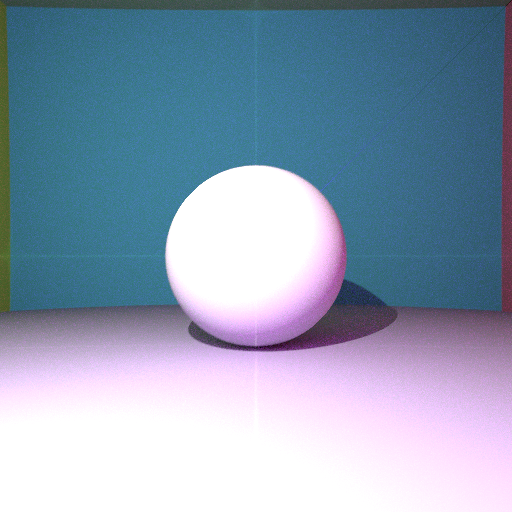
\includegraphics[width=\textwidth]{img/fig2_2.png}
         \caption{With (9.625 seconds)}
     \end{subfigure}
     \caption{A sphere with diffusion, demonstrating indirect lighting. In this picture, the light source was a point.}
\end{figure}

\begin{figure}
     \centering
     \begin{subfigure}[b]{0.49\textwidth}
         \centering
         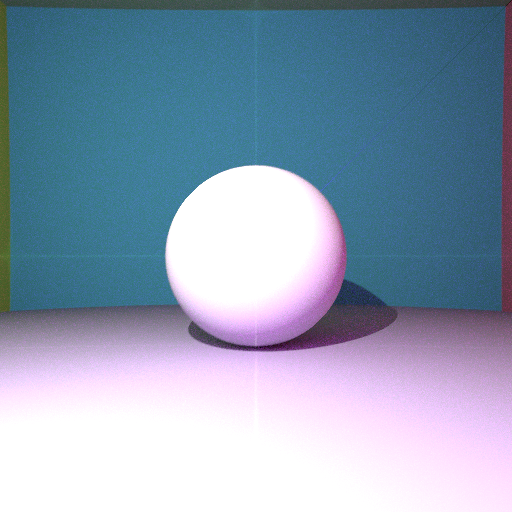
\includegraphics[width=\textwidth]{img/fig2_2.png}
         \caption{Point (9.625 seconds)}
     \end{subfigure}
     \hfill
     \begin{subfigure}[b]{0.49\textwidth}
         \centering
         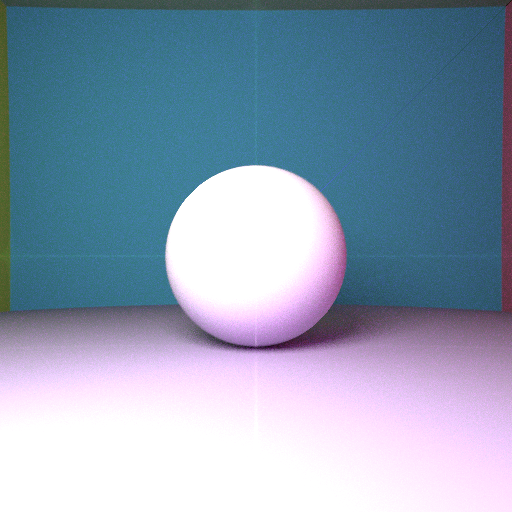
\includegraphics[width=\textwidth]{img/fig3_2.png}
         \caption{Spherical ($r = 10$) (9.035 seconds)}
     \end{subfigure}
     \caption{A sphere with diffusion. Two different light sources were used; indirect lighting was used.}
\end{figure}

\begin{figure}
     \centering
     \begin{subfigure}[b]{0.7\textwidth}
         \centering
         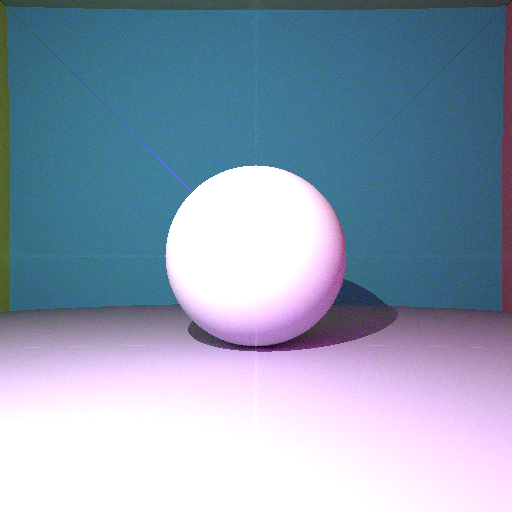
\includegraphics[width=\textwidth]{img/fig4_1.png}
         \caption{Without (16.013 seconds)}
     \end{subfigure}
     \hfill
     \begin{subfigure}[b]{0.7\textwidth}
         \centering
         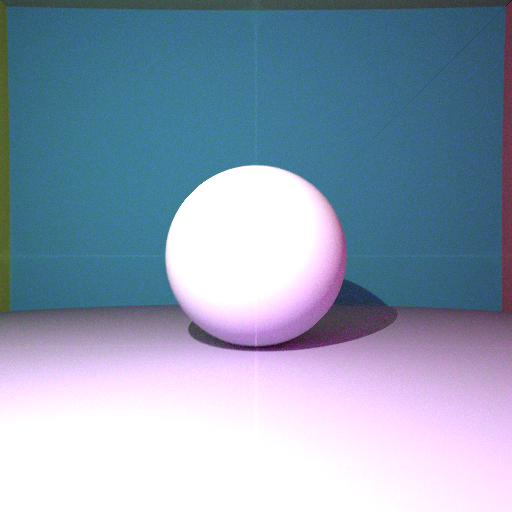
\includegraphics[width=\textwidth]{img/fig4_2.png}
         \caption{With (17.264 seconds)}
     \end{subfigure}
     \caption{A sphere with diffusion, demonstrating antialiasing. In this picture, the light source was a sphere $r = 5$. \emph{No depth of field was used.}}
\end{figure}

\begin{figure}
     \centering
     \begin{subfigure}[b]{0.7\textwidth}
         \centering
         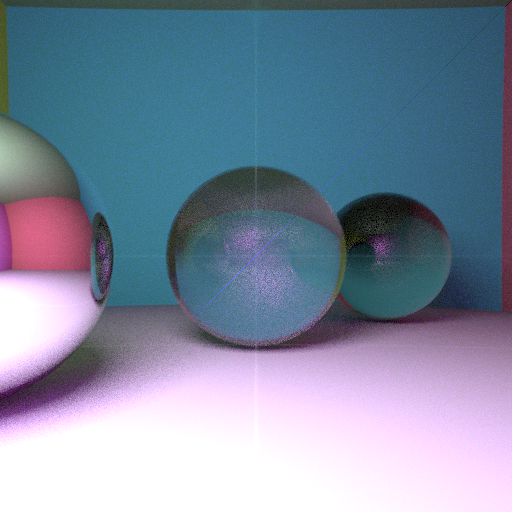
\includegraphics[width=\textwidth]{img/fig5_1.png}
         \caption{Without depth of field (10.925 seconds)}
     \end{subfigure}
     \hfill
     \begin{subfigure}[b]{0.7\textwidth}
         \centering
         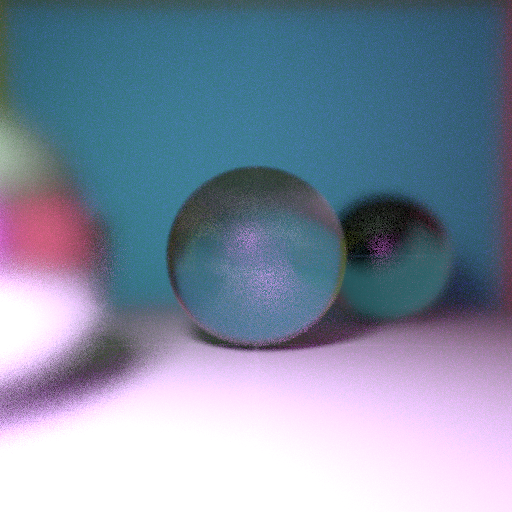
\includegraphics[width=\textwidth]{img/fig5_2.png}
         \caption{With depth of field (12.254 seconds)}
     \end{subfigure}
     \caption{Three balls with reflection, diffusion, and refraction, demonstrating depth of field. In this picture, the light source was a sphere $r = 5$. Refraction was done with Fresnel's law.}
\end{figure}

\begin{figure}
     \centering
     \begin{subfigure}[b]{0.7\textwidth}
         \centering
         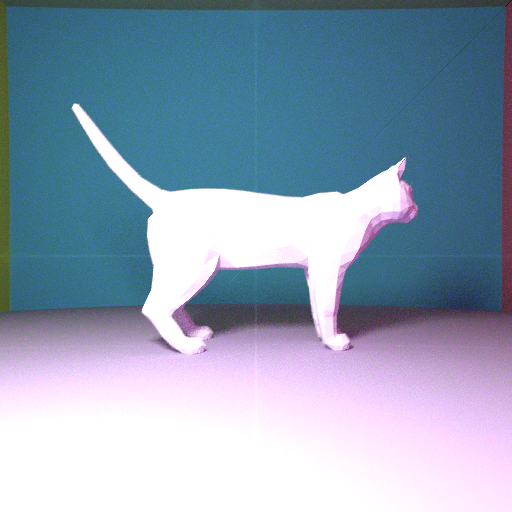
\includegraphics[width=\textwidth]{img/fig6_1.png}
         \caption{Without Phong interpolation (15.153 seconds)}
     \end{subfigure}
     \hfill
     \begin{subfigure}[b]{0.7\textwidth}
         \centering
         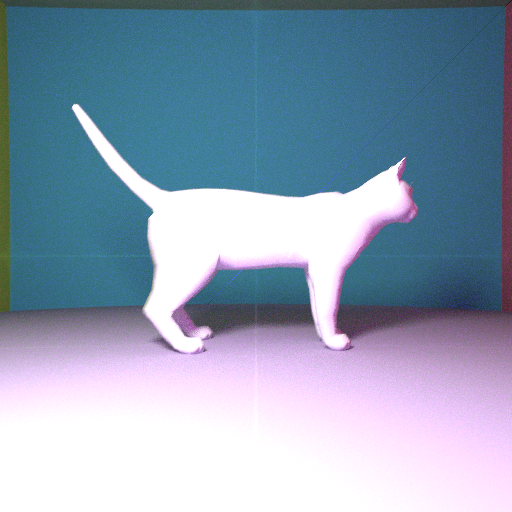
\includegraphics[width=\textwidth]{img/fig6_2.png}
         \caption{With Phong interpolation (14.241 seconds)}
     \end{subfigure}
     \caption{A cat, rendered with BVH and Phong interpolation. In this picture, the light source was a sphere $r = 5$. No depth of field was used to improve visibility.}
\end{figure}

\end{document}
